\documentclass[]{article}
\usepackage{lmodern}
\usepackage{amssymb,amsmath}
\usepackage{ifxetex,ifluatex}
\usepackage{fixltx2e} % provides \textsubscript
\ifnum 0\ifxetex 1\fi\ifluatex 1\fi=0 % if pdftex
  \usepackage[T1]{fontenc}
  \usepackage[utf8]{inputenc}
\else % if luatex or xelatex
  \ifxetex
    \usepackage{mathspec}
  \else
    \usepackage{fontspec}
  \fi
  \defaultfontfeatures{Ligatures=TeX,Scale=MatchLowercase}
\fi
% use upquote if available, for straight quotes in verbatim environments
\IfFileExists{upquote.sty}{\usepackage{upquote}}{}
% use microtype if available
\IfFileExists{microtype.sty}{%
\usepackage{microtype}
\UseMicrotypeSet[protrusion]{basicmath} % disable protrusion for tt fonts
}{}
\usepackage[margin=1in]{geometry}
\usepackage{hyperref}
\hypersetup{unicode=true,
            pdfborder={0 0 0},
            breaklinks=true}
\urlstyle{same}  % don't use monospace font for urls
\usepackage{graphicx}
\makeatletter
\def\maxwidth{\ifdim\Gin@nat@width>\linewidth\linewidth\else\Gin@nat@width\fi}
\def\maxheight{\ifdim\Gin@nat@height>\textheight\textheight\else\Gin@nat@height\fi}
\makeatother
% Scale images if necessary, so that they will not overflow the page
% margins by default, and it is still possible to overwrite the defaults
% using explicit options in \includegraphics[width, height, ...]{}
\setkeys{Gin}{width=\maxwidth,height=\maxheight,keepaspectratio}
\IfFileExists{parskip.sty}{%
\usepackage{parskip}
}{% else
\setlength{\parindent}{0pt}
\setlength{\parskip}{6pt plus 2pt minus 1pt}
}
\setlength{\emergencystretch}{3em}  % prevent overfull lines
\providecommand{\tightlist}{%
  \setlength{\itemsep}{0pt}\setlength{\parskip}{0pt}}
%\setcounter{secnumdepth}{0}
% Redefines (sub)paragraphs to behave more like sections
\ifx\paragraph\undefined\else
\let\oldparagraph\paragraph
\renewcommand{\paragraph}[1]{\oldparagraph{#1}\mbox{}}
\fi
\ifx\subparagraph\undefined\else
\let\oldsubparagraph\subparagraph
\renewcommand{\subparagraph}[1]{\oldsubparagraph{#1}\mbox{}}
\fi

%%% Use protect on footnotes to avoid problems with footnotes in titles
\let\rmarkdownfootnote\footnote%
\def\footnote{\protect\rmarkdownfootnote}

%%% Change title format to be more compact
\usepackage{titling}

% Create subtitle command for use in maketitle
\newcommand{\subtitle}[1]{
  \posttitle{
    \begin{center}\large#1\end{center}
    }
}

\setlength{\droptitle}{-2em}
  \title{}
  \pretitle{\vspace{\droptitle}}
  \posttitle{}
  \author{}
  \preauthor{}\postauthor{}
  \date{}
  \predate{}\postdate{}

\usepackage{float}
\usepackage[labelfont=bf]{caption}
\usepackage[labelfont=bf, justification=justified]{subcaption}
\captionsetup{position=top}
\captionsetup[subfigure]{justification=centering}

\graphicspath{{./Figuras/}}
\usepackage{epstopdf}
\epstopdfDeclareGraphicsRule{.tiff}{png}{.png}{convert #1 \OutputFile}
\AppendGraphicsExtensions{.tiff}

\begin{document}

\section{Motivation}\label{motivation}

Mexican labour courts face a large and growing backlog of cases. The
backlog is made worse by case settlement rates that are low by
international standards. Our previous work suggests that one cause of
the low settlement rates is that parties are overconfident of their
chances of success. We tested this hypothesis through an experimental
intervention in the Mexico City Labour Court (MCLC). In a pilot project
in the MCLC, we provided objective statistical information to parties in
randomly selected cases to see if this information changed the
likelihood of parties reach a settlement. An initial 12-week pilot in
one of the MCLC's 20 subcourts showed that providing objective
information nearly doubled settlement rates on the same day. Given these
initial results, we then increased the scale of the project for a second
intervention to confirm the result.

These experiments required that we generate information to share with
workers. We produced a set of predictive models using data from cases
filed in 2011.We refer to the resulting product as a ``calculator.'' The
predicted outcomes are based on information in case filings, including
the wage and tenure of the worker, and other variables described in more
detail below. Each of the MCLC's 20 subcourts handles cases originating
from disputes in a given set of industries. Thus, the predictive
information needed to be based on information from the relevant
subcourts.

For the initial experiment, we used data from cases filed in 2011 in
subcourt 7, where the pilot took place; for the second experiment, we
revised the calculator based on information from the five subcourts
where the expanded experiment took place. In both cases, we used data on
whether the case was completed or still ongoing, and the amount of any
settlement for the subset of lawsuits that were settled. The calculator
produces predictions on the probability of the case finishing with a
certain outcome and the expected payoff of that outcome (this includes
the amount of money awarded to the plaintiff and the overall duration of
the lawsuit).

\section{First Pilot}\label{first-pilot}

\subsection{Our questions}\label{our-questions}

We aimed to provide three pieces of information:

\begin{enumerate}
\def\labelenumi{\arabic{enumi}.}
\item
  How likely is settlement, abandonment by the plaintiff, expiry, or a
  judicial decision in favour of either party?
\item
  Given a particular outcome, what was the expected duration for the
  entire process?
\item
  Given a particular outcome, what was the expected compensation at the
  end of the process?
\end{enumerate}

These questions were addressed as one classification problem -for the
first case- and two regression/prediction problems -for the second and
third cases.

\subsection{Data}\label{data}

The data for our first calculator came from a sample of 1000 concluded
case files from a single subcourt (subcourt 7). Defendants in subcourt 7
consist mostly of outsourcing, transportation firms and gas stations.

We coded data directly from casefiles, and then randomly inspected 20\%
of the data entries by comparing the manually coded databases against
the actual casefiles to ensure that the initial coding was accurate. Our
data cleaning process was fairly standard. We then examined the data for
outliers, recoding as necessary We excluded a small number of cases for
which key information was missing.

\subsection{Models}\label{models}

For all three questions, the sample was divided in 70-30 training and
test sets. We simplified categorical variables in order to remove sparse
groups in our covariates.

\subsubsection{Discrete outcomes}\label{discrete-outcomes}

We aggregated the ending possibilites for casefiles into 5 different
outcomes:

\begin{itemize}
\item
  Settlement
\item
  Expiry
\item
  Court Ruling with a positive compensation
\item
  Court Ruling with no compensation
\item
  Drop
\end{itemize}

The dependent variable -a categorical variable depicting the case
ending- was recoded into 5 dummy variables. The following models were
then tested for classification of each binary outcome:

\begin{itemize}
\item Logistic Regression

\item Probit

\item Random Forest (100 trees)

\item Single-hidden-layer Neural Network (20 nodes in the hidden layer and 10\% weight decay)

\item Gradient Boosting
\end{itemize}

Due to our sample size, all hyperparameters were chosen specifically to
avoid overfitting. Models were chosen for each outcome based on
classification accuracy for the test set. Figure \ref{accuracy_scores} shows the classification accuracy rates of all our final discrete models.

\begin{figure}[H]
   \caption{Accuracy scores by binary outcome}
   \label{accuracy_scores}
    \begin{center}
    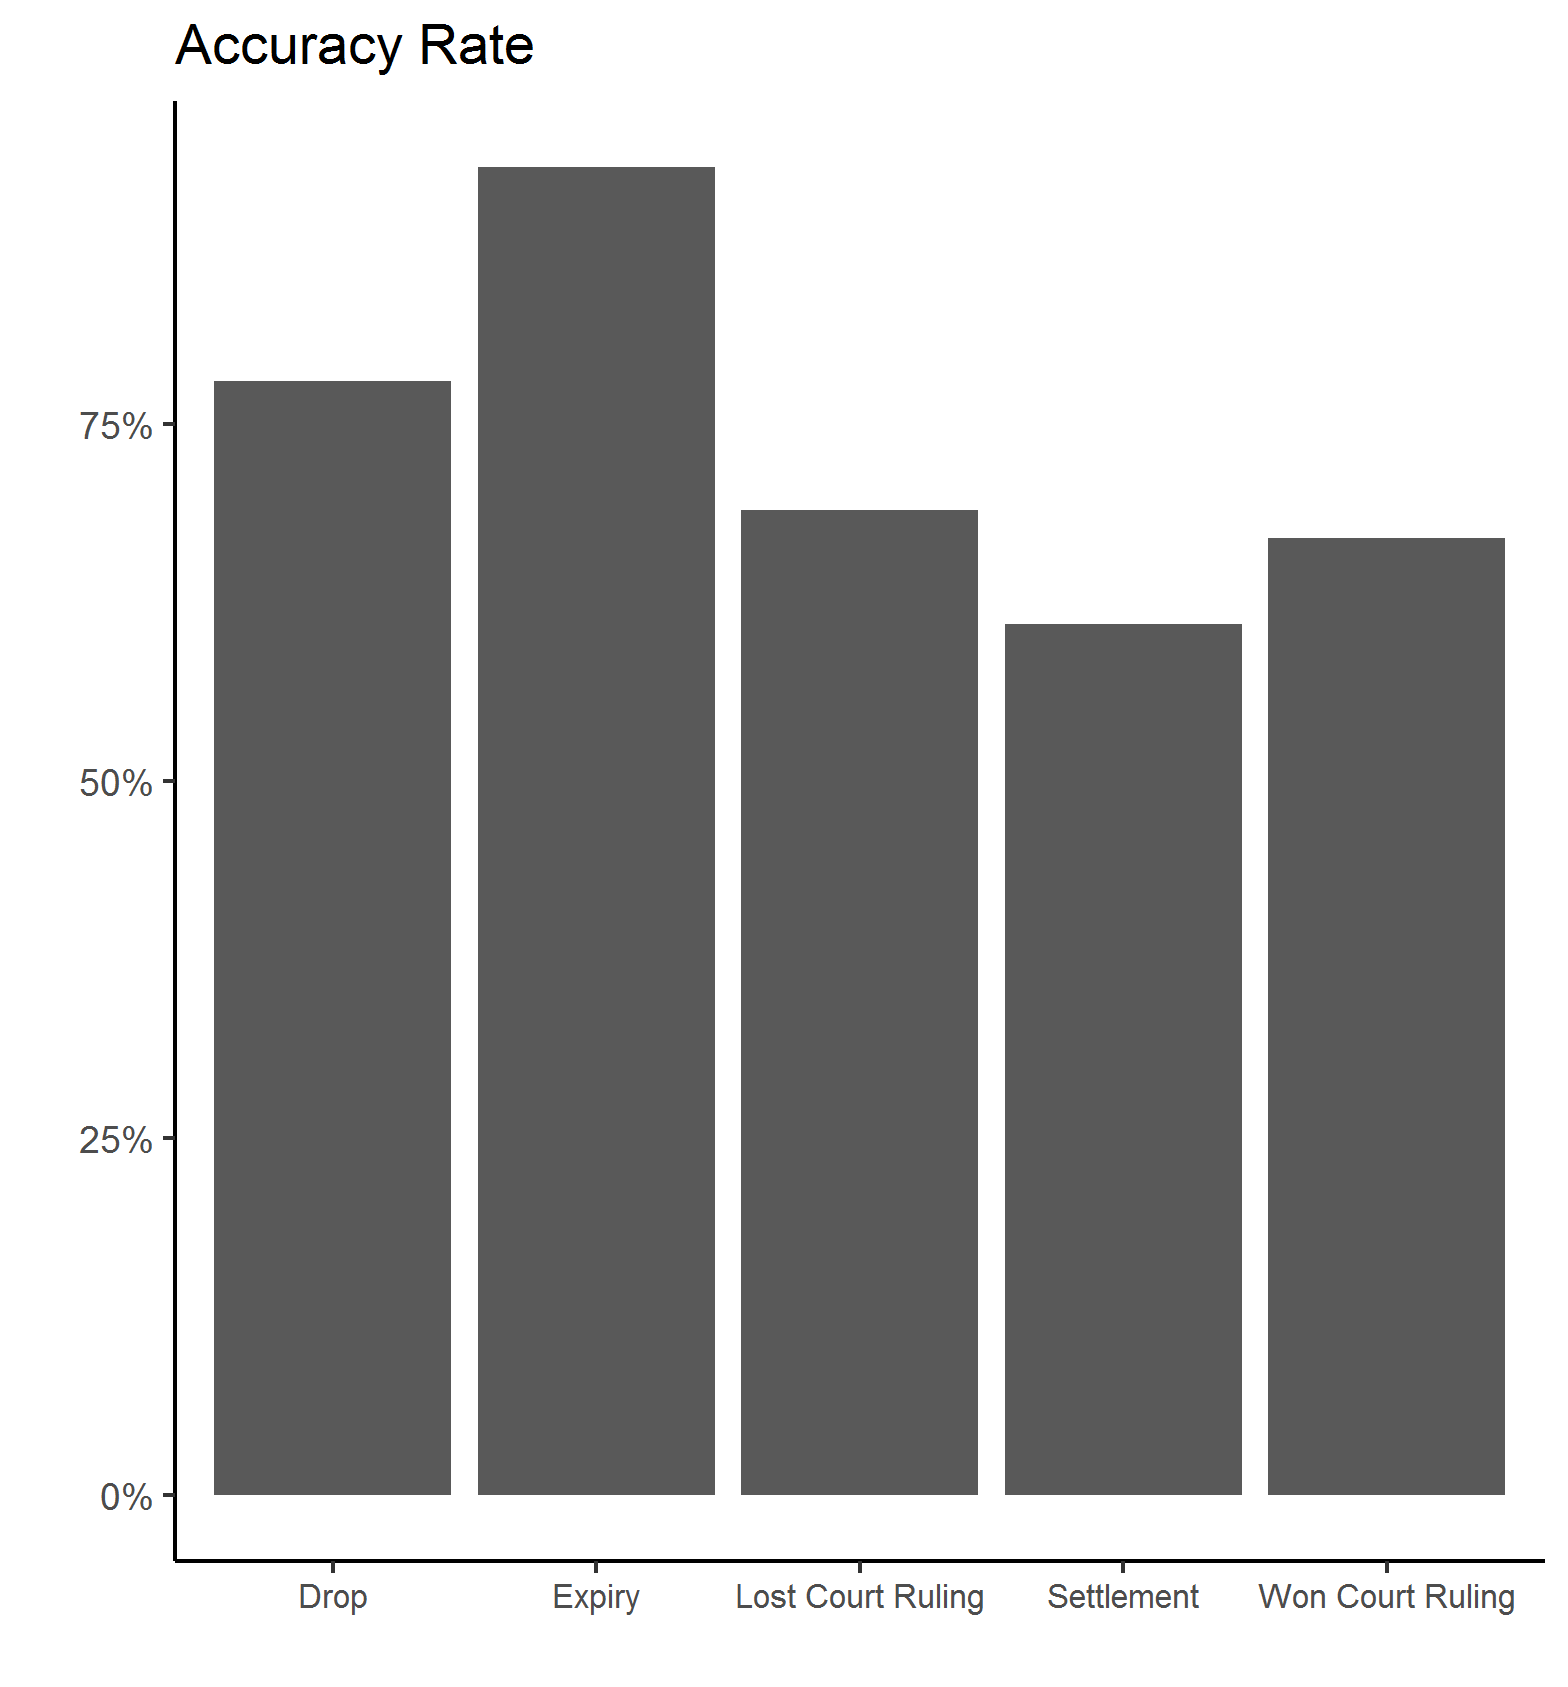
\includegraphics[width=0.3\textwidth]{oos_fit_categorical.tiff}
    \end{center}
\end{figure}

\subsubsection{Continuous outcomes}\label{continuous-outcomes}

We set out to predict expected lawsuit duration for each given outcome.
Predicting expected compensation was only required for Settlements and
Court Rulings, since the other outcomes imply zero expected payment. We
trained a set of 4 different models for each prediction problem,
considering both regular and logarithmic models. The logarithmic models
proved extremely useful to tackle the skewness of our dependent variable
distributions. Our model list included the following:

\begin{itemize}
\item OLS regression

\item GLM Boosting

\item Random Forest (100 trees)

\item Ridge Regression
\end{itemize}

The 7 models to be used in the calculator were chosen based on the \emph{MAPD (Mean Absolute Percentage Deviation).} This evaluation
measure was chosen because we had no zero values in our dependent
variables and were inclined to giving rather conservative predictions to
parties. Figures \ref{duration_predictions} and \ref{compensation_predictions} show the out-of-sample fit for every final continuous model. For each model, we regress the prediction on our dependent variable and show the $R^2$ in the plot subtitle.

\begin{figure}[H]
    \caption{Duration predictions in the first pilot}
    \label{duration_predictions}
    \begin{center}
    \begin{subfigure}{0.49\textwidth}
    \centering
        \includegraphics[width=.75\textwidth]{mod_duracion_caducidad.tiff}
     \end{subfigure}
     \begin{subfigure}{0.49\textwidth}
    \centering
        \includegraphics[width=.75\textwidth]{mod_duracion_convenio.tiff}
     \end{subfigure}
     \hfill
         \begin{subfigure}{0.49\textwidth}
    \centering
        \includegraphics[width=.75\textwidth]{mod_duracion_laudo_pierde.tiff}
     \end{subfigure}
     \begin{subfigure}{0.49\textwidth}
    \centering
        \includegraphics[width=.75\textwidth]{mod_duracion_laudo_gana.tiff}
     \end{subfigure}
     \hfill
         \begin{subfigure}{0.49\textwidth}
    \centering
        \includegraphics[width=.75\textwidth]{mod_duracion_desiste.tiff}
     \end{subfigure}
        \end{center}
        %{\footnotesize \textit{Notes: } Scatter plot of compensation predictions and outcomes }
\end{figure}


\begin{figure}[H]
    \caption{Compensation predictions in the first pilot}
    \label{}
    \begin{center}
    \begin{subfigure}{0.49\textwidth}
    \centering
        \includegraphics[width=.75\textwidth]{mod_liqtotal_convenio.tiff}
     \end{subfigure}
     \begin{subfigure}{0.49\textwidth}
    \centering
        \includegraphics[width=.75\textwidth]{mod_liqtotal_laudo_gana.tiff}
     \end{subfigure}
  \end{center}
    %    {\footnotesize \textit{Notes: } Scatter plot of compensation predictions and outcomes }
\end{figure}


\subsection{Display of Information}\label{display-of-information}

Our prediction sheets were generated for each subject in real time, and
contained the following information:

\begin{figure}[H]
\centering
\caption{Information sheet in the first pilot (shown to both parties)}
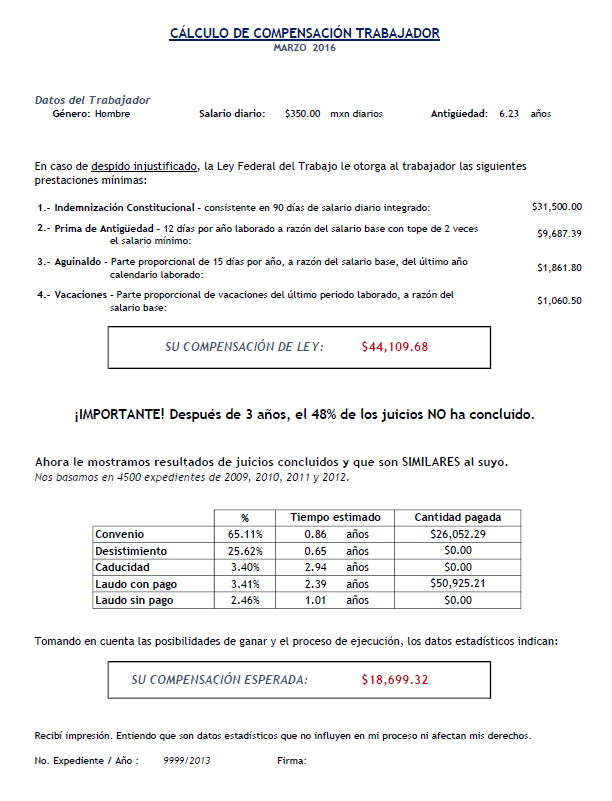
\includegraphics{calctreat.png}
\end{figure}

\pagebreak

\section{Scale-Up}\label{scale-up}

\subsection{Our Questions}\label{our-questions-1}

We narrowed our original set of questions to answering:

\begin{enumerate}
\def\labelenumi{\arabic{enumi}.}
\item
  Given a case ending in a court ruling, how likely is to recover a
  positive compensation?
\item
  What would be that expected compensation?
\item
  Given a case ending in settlement, what would be the expected
  compensation?
\end{enumerate}

\subsection{Data}\label{data-1}

This scale-up was running in 5 different subcourts -including subcourt
7- so we coded an additional 4000 casefiles from the new subcourts, from
the same time period. We used all 5000 observations as our working data.
The coding and supervision process was entirely analogous to the ones
implemented in our first pilot.

\subsection{Models}\label{models-1}

The operation of the first pilot gave us two key insights for building
our second calculator: we wanted to display less information for
subjects to process, and we were to stress the relationship between the
subject and the information we were sharing, so we decided to limit our
predictions and include some personalized information on the worker,
intended to shed some light on the drivers of our predictions.

\subsubsection{Discrete outcomes}\label{discrete-outcomes-1}

Our classification problem became slightly different. In order to assess
the unbalancedness of our court rulings sample -only 24\% of court
rulings ever recover something- we used a Synthetic Minority
Over-Sampling Technique (see
\href{http://jair.org/media/953/live-953-2037-jair.pdf}{Chawla et.al., 2002}) and did a 80-20 train vs.~test split on our
data.

After some preliminary tests, we decided to focus on Random Forests. For
this Scale-Up, we perfomed grid search in order to find the best
hyperparameter setting. We compared 7 different models with the number
of trees ranging between 900 and 1500.

Our final model resulted in a Random Forest of 1200 CARTs, which yielded
an 86\% accuracy rate on test classification.

\subsubsection{Continuous outcomes}\label{continuous-outcomes-1}

In order for our results to be easily interpreted and taking advantage
of our bigger sample size, we decided to use more standard regression
tools. We compared between several specifications of OLS and Kernel
regressions, using a Gaussian kernel for the latter. Both models were
trained for the original variables and taking logarithms of all numeric
variables.

The final models were chosen based on the Mean Squared Error, and
certain aspects of the out-of-sample error distributions. For this
second criterion we estimated this distribution by retraining the model
1000 times on a 70-30 train-test split and computing prediction errors. Figure \ref{continuous_predictions} shows the out-of-sample fit for our continuous models. For each model, we regress the prediction on our dependent variable and show the $R^2$ in the plot subtitle. 

\begin{figure}[H]
    \caption{Compensation predictions in the second pilot}
    \label{continuous_predictions}
    \begin{center}
    \begin{subfigure}{0.49\textwidth}
    \centering
        \includegraphics[width=.75\textwidth]{prediction_convenio.tiff}
     \end{subfigure}
     \begin{subfigure}{0.49\textwidth}
    \centering
        \includegraphics[width=.75\textwidth]{prediction_laudo.tiff}
     \end{subfigure}
  \end{center}
        %{\footnotesize \textit{Notes: } Scatter plot of compensation predictions and outcomes }
\end{figure}



\subsection{Display of Information}\label{display-of-information-1}

The information sheets were generated before time for this operation,
and handed out to subjects in treatment days. The sheets had the
following layout:

\begin{figure}[H]
\centering
\caption{Information sheet for plaintiff}
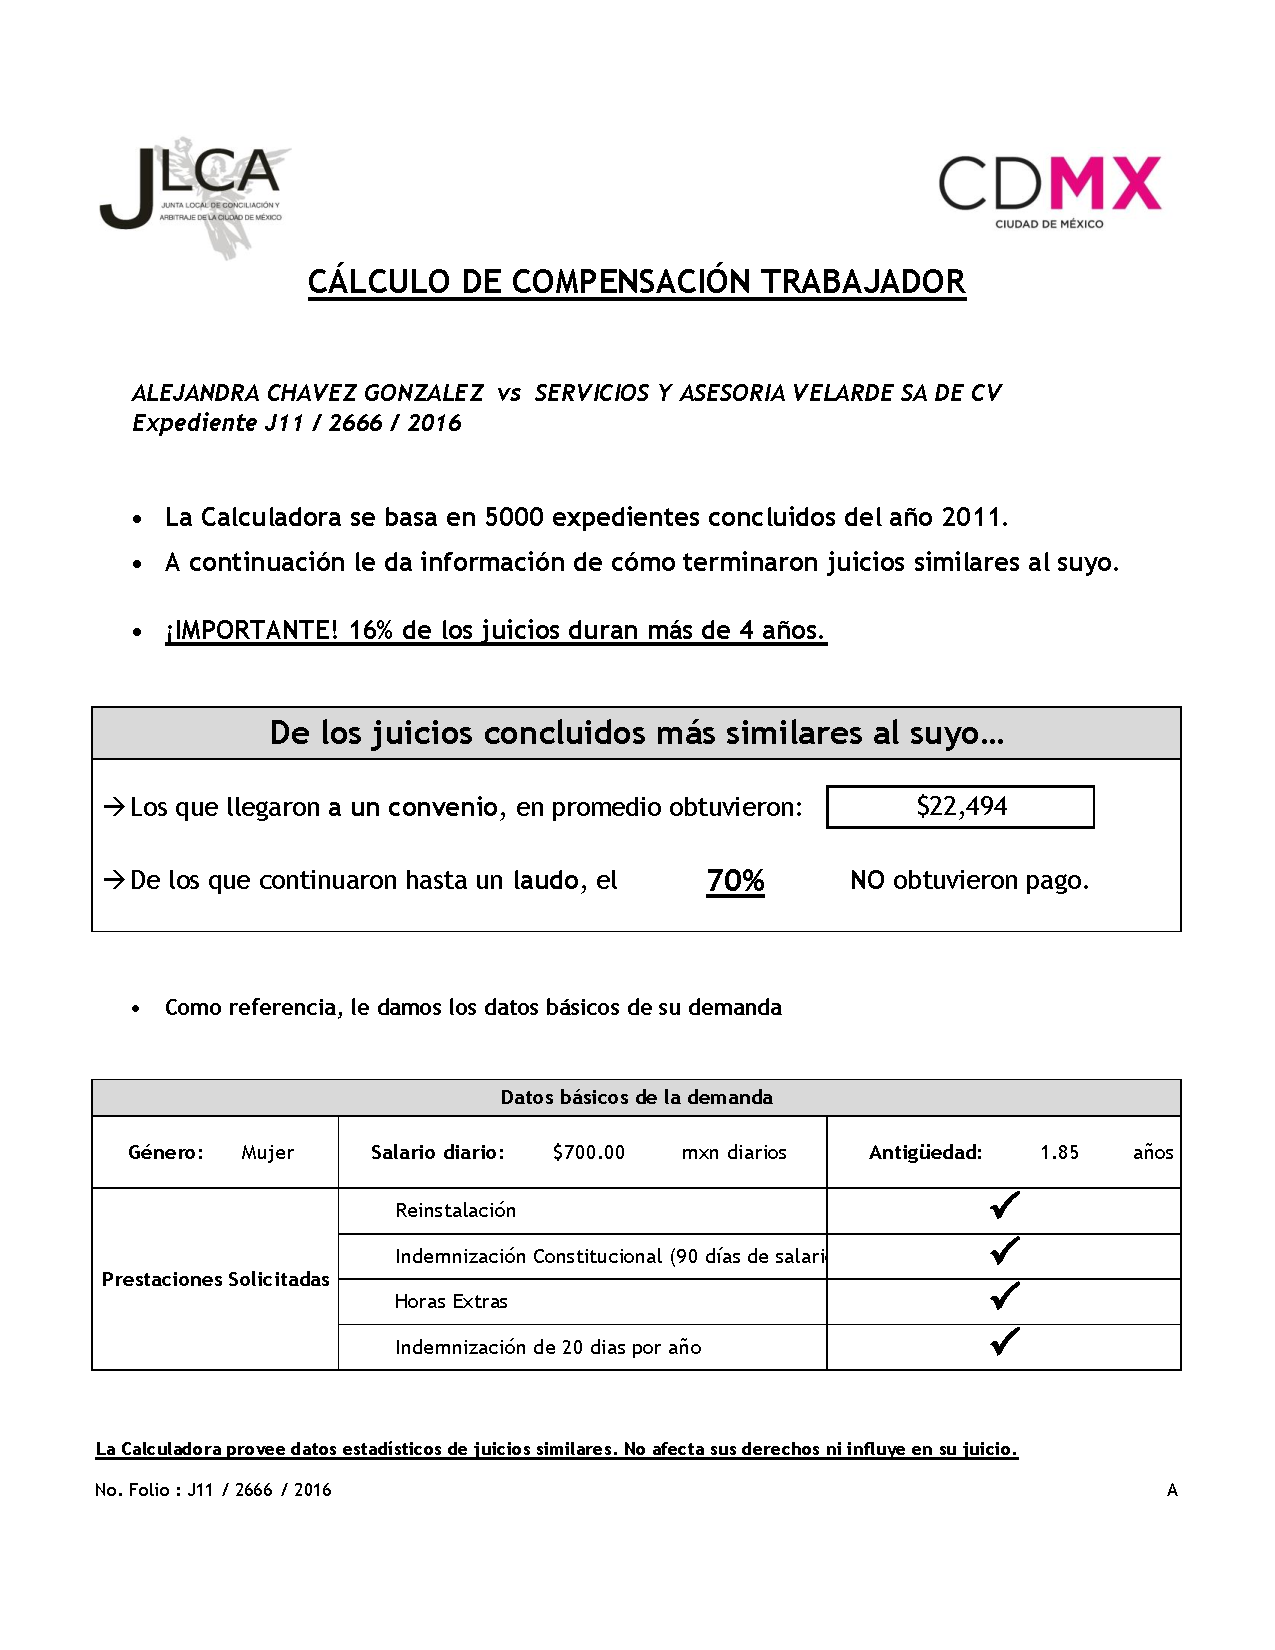
\includegraphics[width=.75\textwidth]{calctreat_act.pdf}

\end{figure}


\begin{figure}[H]
\centering
\caption{Information sheet for defendant}
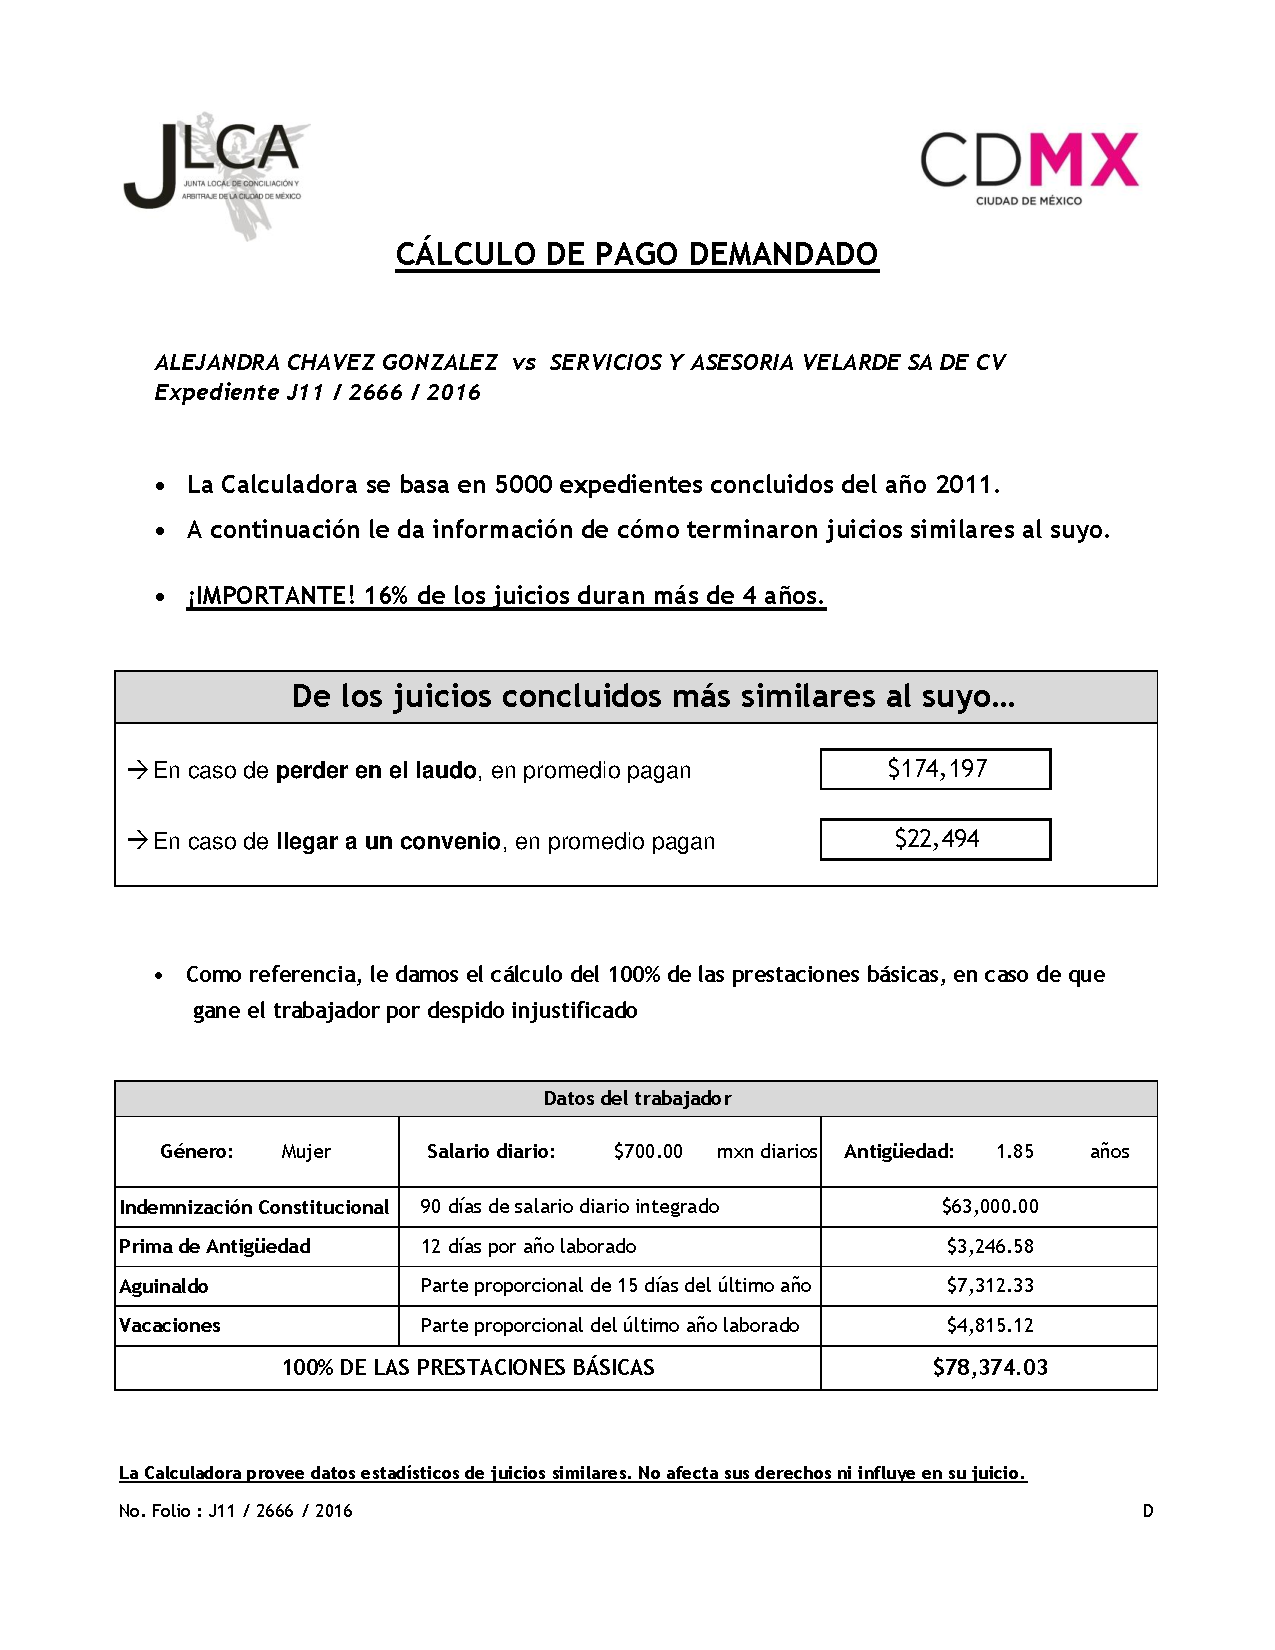
\includegraphics[width=.75\textwidth]{calctreat_dem.pdf}

\end{figure}

\end{document}

